%\documentclass[handout,xcolor=svgnames]{beamer}
\documentclass[xcolor=svgnames]{beamer}
\usepackage[utf8]{inputenc}
\usepackage[english]{babel}
\usepackage{transparent}
\usepackage{booktabs}
\usepackage{xcolor}
\usepackage{numprint}


\makeatletter
\newbox\@backgroundblock
\newenvironment{backgroundblock}[2]{%
  \global\setbox\@backgroundblock=\vbox\bgroup%
    \unvbox\@backgroundblock%
    \vbox to0pt\bgroup\vskip#2\hbox to0pt\bgroup\hskip#1\relax%
}{\egroup\egroup\egroup}
\addtobeamertemplate{background}{\box\@backgroundblock}{}
\makeatother

\usetheme{Proso}

\title[Choosing a Student Model for a Real World
Application]{Choosing a Student Model for a Real World
Application}
\author{\textbf{Ji\v{r}í \v{R}ihák}, Radek Pelánek}
\institute{Masaryk University Brno}
\date{}

\begin{document}
% --------------------------- SLIDE --------------------------------------------
\frame[plain]{\titlepage}
% ------------------------------------------------------------------------------
% --------------------------- SLIDE --------------------------------------------
\begin{frame}
    Development of applications: matmat.cz, outlinemaps.org, \dots
    \begin{itemize}
        \item Which student model to choose
        \item How to set parameters
        \item How many answers model needs
        \item \dots
    \end{itemize}
\end{frame}
% ------------------------------------------------------------------------------
% --------------------------- SLIDE --------------------------------------------
\begin{frame}
    \frametitle{matmat.cz}

    \begin{backgroundblock}{15mm}{15mm}
        \hspace{0.6\linewidth}
        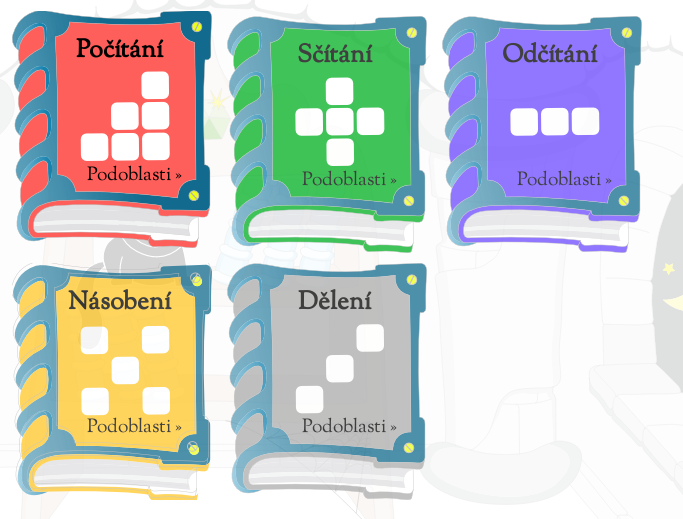
\includegraphics[width=0.3\linewidth]{figures/matmat2}
     \end{backgroundblock}

    \begin{backgroundblock}{15mm}{45mm}
        \hspace{0.6\linewidth}
        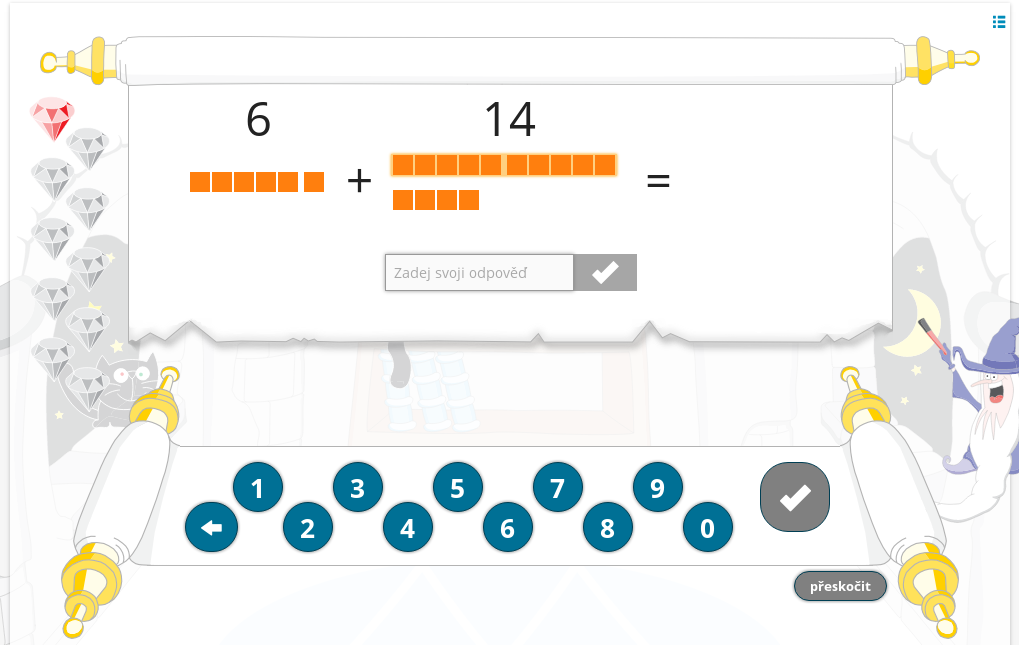
\includegraphics[width=0.3\linewidth]{figures/matmat}
     \end{backgroundblock}

    \begin{itemize}
        \item online, free, without ads
        \item basic arithmetic - $ +, -, \times, \div$
        \item \numprint{150000} answers, \numprint{2000} items
        \item adaptive practice
        \item importance of response time
        \only<2>{
        \begin{itemize}
            \item correct answer to $3 \times 5 $ in \textbf{2} seconds
            \item correct answer to $3 \times 5 $ in \textbf{14} seconds
        \end{itemize}
        }
    \end{itemize}
\end{frame}
% ------------------------------------------------------------------------------
% --------------------------- SLIDE --------------------------------------------
\begin{frame}
    \frametitle{Adaptability}
    \begin{itemize}
        \item selection of question - targeting 75\% success rate
        \item model parameters - \textbf{difficulties} of items and \textbf{skills} of learners
        \item domain model - several skills per learner
        \item use of response time
    \end{itemize}

    \vfill

    \centering
    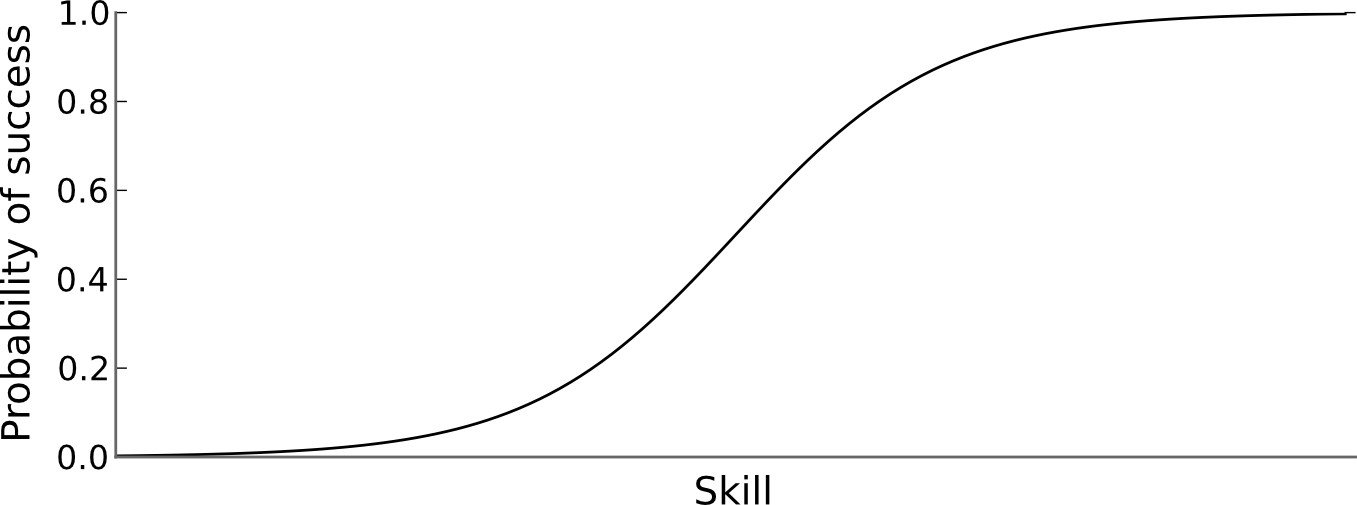
\includegraphics[width=0.6\linewidth]{figures/logistic}
\end{frame}
% ------------------------------------------------------------------------------
% --------------------------- SLIDE --------------------------------------------
\begin{frame}
    \centering

    \huge
    What aspects of student modeling are most important?

\end{frame}
% ------------------------------------------------------------------------------
% --------------------------- SLIDE --------------------------------------------
\begin{frame}
    \frametitle{Aspects to Compare}

    Three aspects of student modeling
    \begin{itemize}
        \item domain models
        \item response times uses
        \item missing answers
    \end{itemize}

\end{frame}
% ------------------------------------------------------------------------------
% --------------------------- SLIDE --------------------------------------------
\begin{frame}
    \frametitle{Domain Modeling}
    \centering
    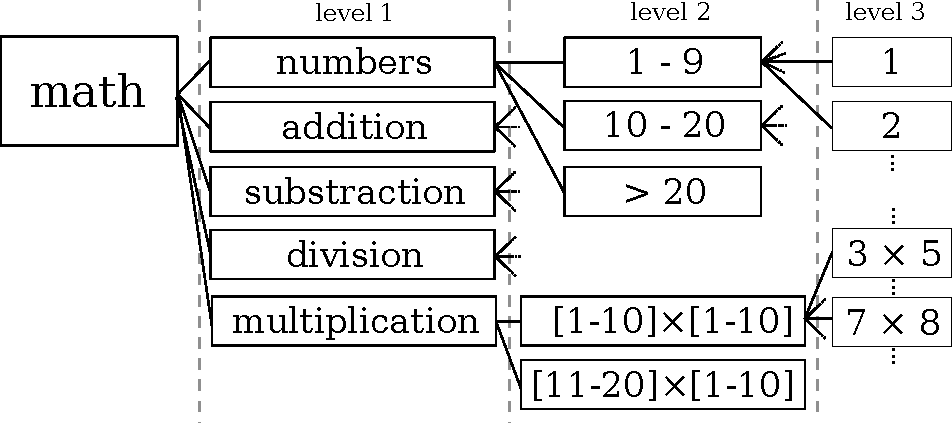
\includegraphics[width=0.9\linewidth]{figures/domain-models}

    \vfill
    \huge
    \only<2>{ Too complicated? }

\end{frame}
% ------------------------------------------------------------------------------
% --------------------------- SLIDE --------------------------------------------
\begin{frame}
    \frametitle{Domain Modeling}

    \begin{itemize}
        \item Item average - no skill
        \only<2->{ \item Basic model - one global skill}
        \only<3->{ \item Concepts model - 5 skills}
        \only<4->{ \item Hierarchical model}
    \end{itemize}

    \vfill
    \centering
    \only<1>{  \phantom{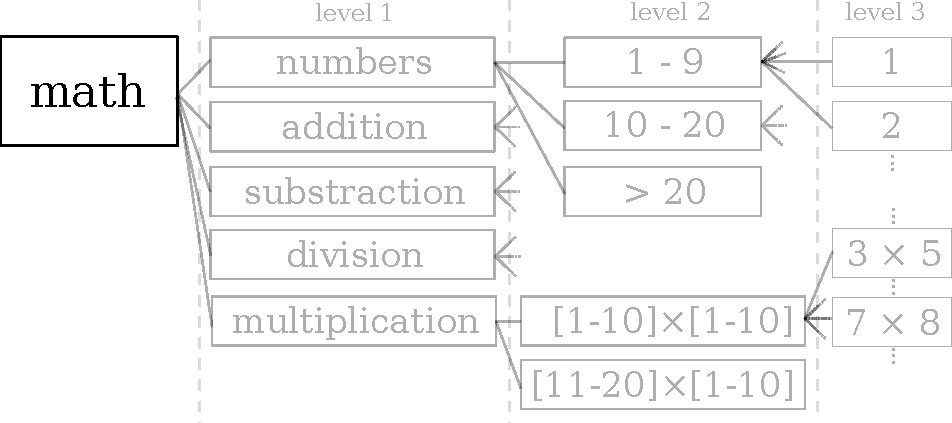
\includegraphics[width=0.6\linewidth]{figures/domain-models-global}}}
    \only<2>{  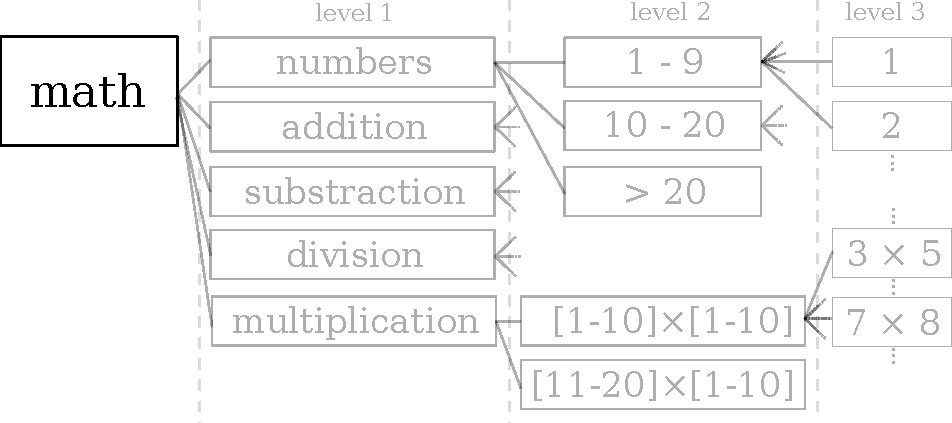
\includegraphics[width=0.6\linewidth]{figures/domain-models-global}}
    \only<3>{  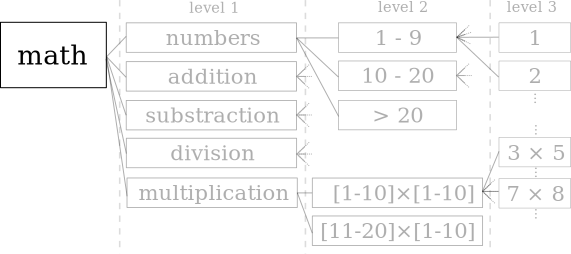
\includegraphics[width=0.6\linewidth]{figures/domain-models-concepts}}
    \only<4>{  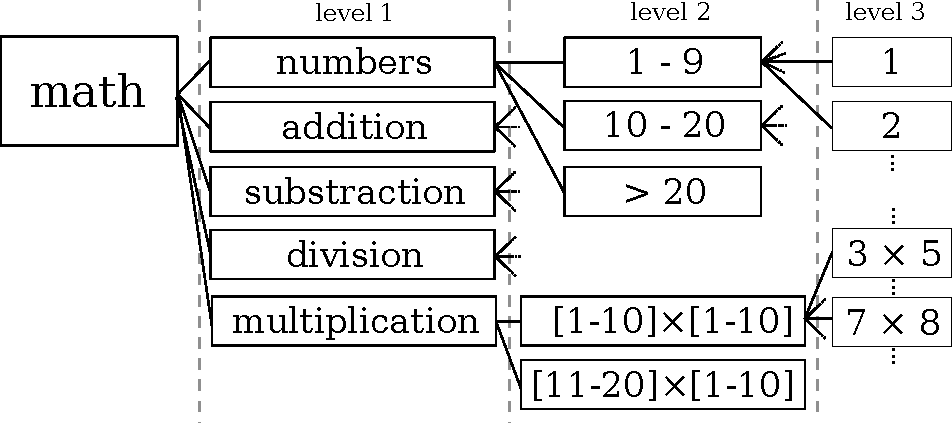
\includegraphics[width=0.6\linewidth]{figures/domain-models}}

\end{frame}
% ------------------------------------------------------------------------------
% --------------------------- SLIDE --------------------------------------------
\begin{frame}
    \frametitle{Response Times}

    \begin{itemize}
        \item classic response:
            \begin{itemize}
                \item $r = 0$ - wrong answer
                \item $r = 1$ - correct answer
            \end{itemize}
        \item use of response time:
            \begin{itemize}
                \item $r = 0$ - wrong answer
                \item $r \in [0, 1]$ - correct answer
            \end{itemize}
    \end{itemize}

\end{frame}
% ------------------------------------------------------------------------------
% --------------------------- SLIDE --------------------------------------------
\begin{frame}
    \frametitle{Response Times}

    \begin{itemize}
        \item \textcolor{blue}{no time}
        \item \textcolor{green}{threshold time}
        \item \textcolor{red}{exponential time}
        \item \textcolor{violet}{linear time}
    \end{itemize}

    \vfill
    \centering
    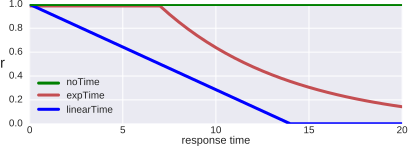
\includegraphics[width=0.9\linewidth]{figures/time-uses}

\end{frame}
% ------------------------------------------------------------------------------
% --------------------------- SLIDE --------------------------------------------
\begin{frame}
    \frametitle{Wrong Answers}

    \begin{itemize}
        \item many missing answers - skips
        \item long sequences of missing answers
        \begin{itemize}
            \item adults trying system
            \item gaming system
        \end{itemize}
        \item simple model extension:
        \begin{itemize}
            \item probability of missing next answer
            \item based on number of previous missing answers
        \end{itemize}
    \end{itemize}
\end{frame}
% ------------------------------------------------------------------------------
% --------------------------- SLIDE --------------------------------------------
\begin{frame}
    \frametitle{Aspects to Compare}

    Three aspects of student modeling
    \begin{itemize}
        \item domain models - 4
        \item response times uses - 4
        \item missing answers - with and without
    \end{itemize}

\end{frame}
% ------------------------------------------------------------------------------
% --------------------------- SLIDE --------------------------------------------
\begin{frame}
    \frametitle{Prediction Accuracy}

    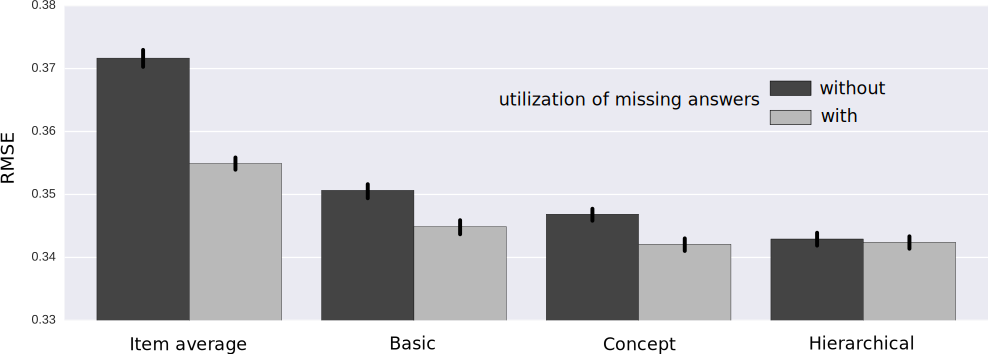
\includegraphics[width=\linewidth]{figures/missing-answers}

    \begin{enumerate}
        \item Large improvement over baseline does not mean usefulness for more complex models.
    \end{enumerate}
\end{frame}
% ------------------------------------------------------------------------------
% --------------------------- SLIDE --------------------------------------------
\begin{frame}
    \frametitle{Prediction Accuracy - Time}

    Comparing models with different time utilization
    \begin{itemize}
        \item models are trained to predict different absolute values
        \item direct comparison is not possible
    \end{itemize}
\end{frame}
% ------------------------------------------------------------------------------
% --------------------------- SLIDE --------------------------------------------
\begin{frame}
    \frametitle{Estimated Parameters - Difficulties}

    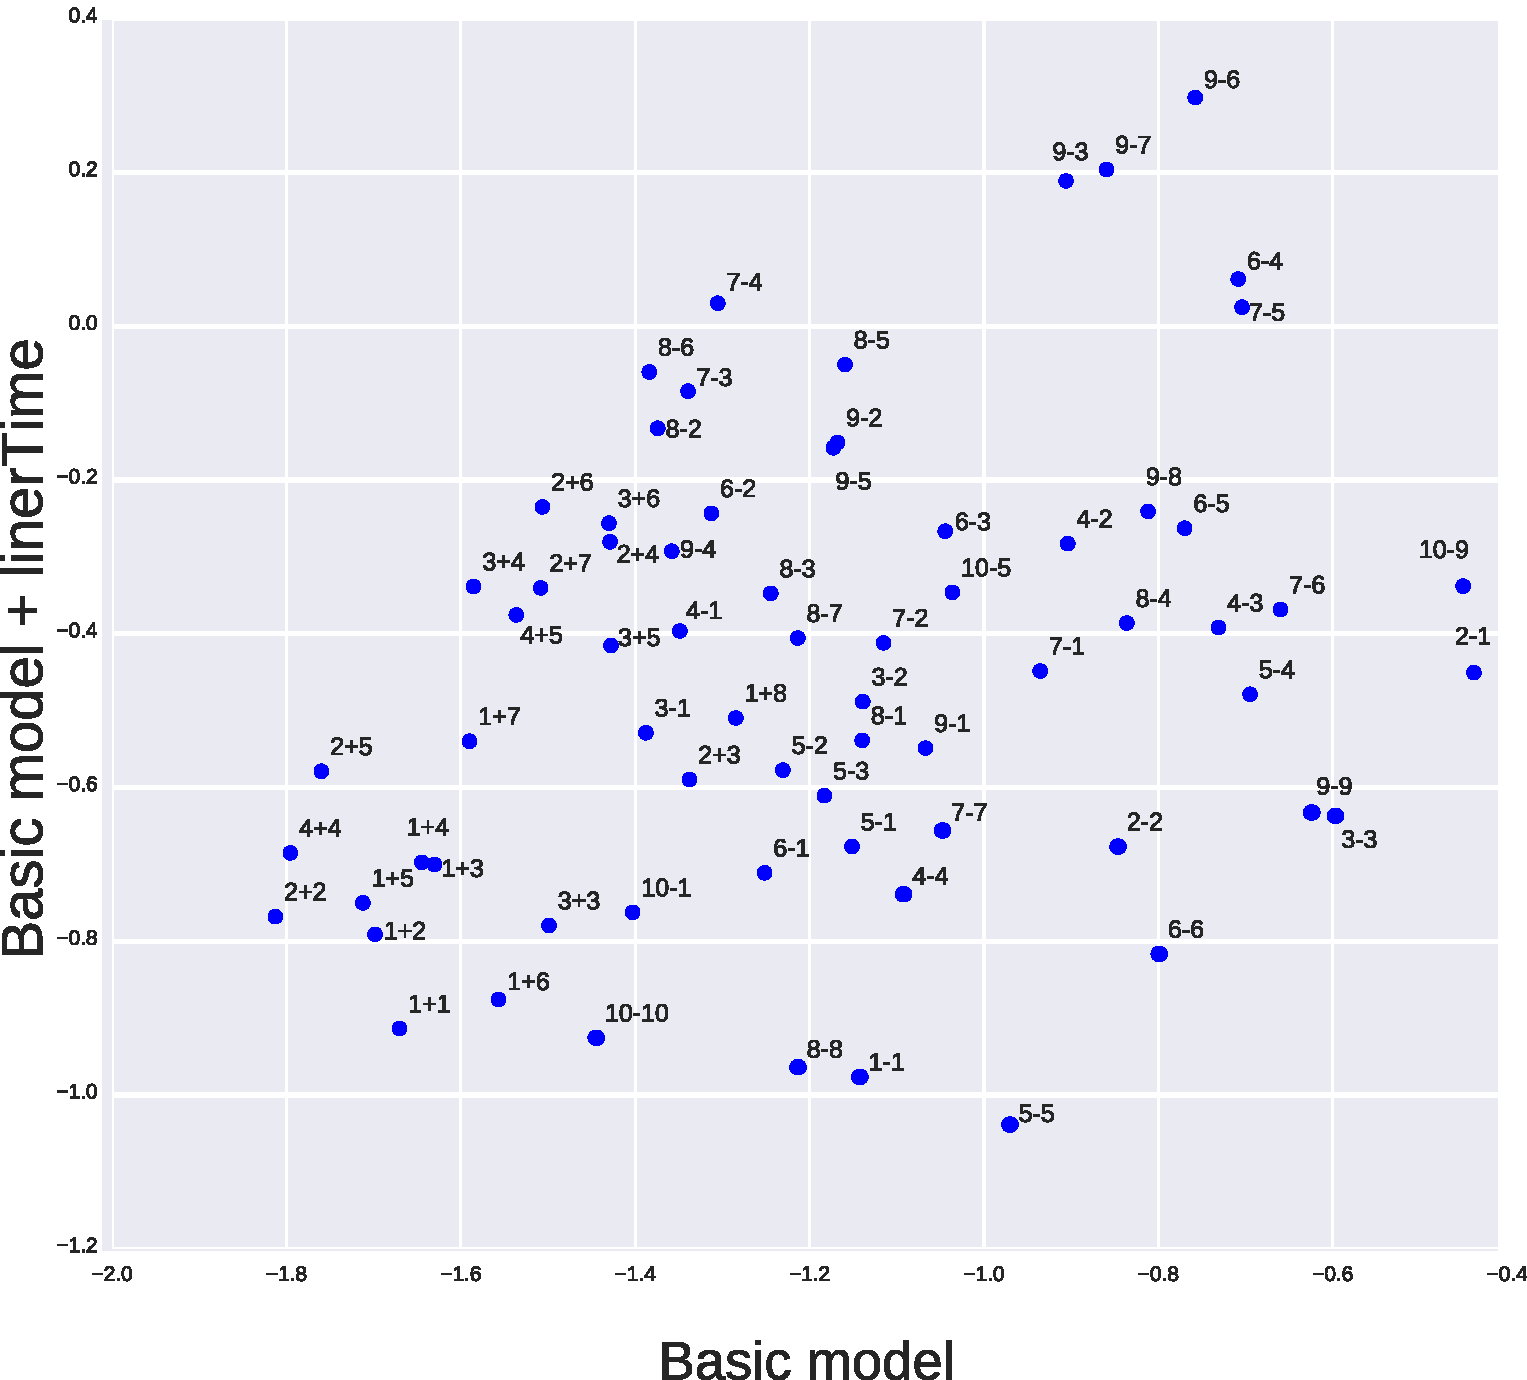
\includegraphics[width=\linewidth]{figures/difficulties-one-color}
\end{frame}
% ------------------------------------------------------------------------------
% --------------------------- SLIDE --------------------------------------------
\begin{frame}
    \frametitle{Correlations of Estimated Parameters}
    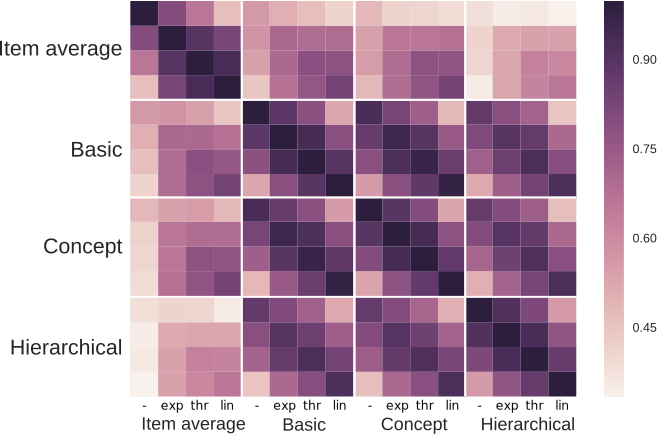
\includegraphics[width=\linewidth]{figures/difficulty-correlations}
\end{frame}
% ------------------------------------------------------------------------------
% --------------------------- SLIDE --------------------------------------------
\begin{frame}
    \frametitle{Correlations of Estimated Parameters}
    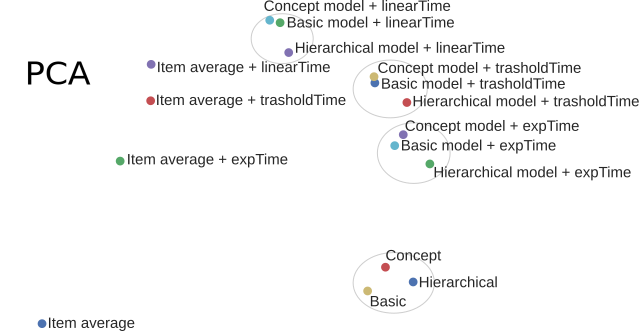
\includegraphics[width=\linewidth]{figures/pca}
    \begin{enumerate}
        \setcounter{enumi}{1}
        \item Response time utilization have larger impact on trained parameters that domain modeling.
    \end{enumerate}
\end{frame}
% ------------------------------------------------------------------------------
% --------------------------- SLIDE --------------------------------------------
\begin{frame}
    \frametitle{Estimated Parameters}
    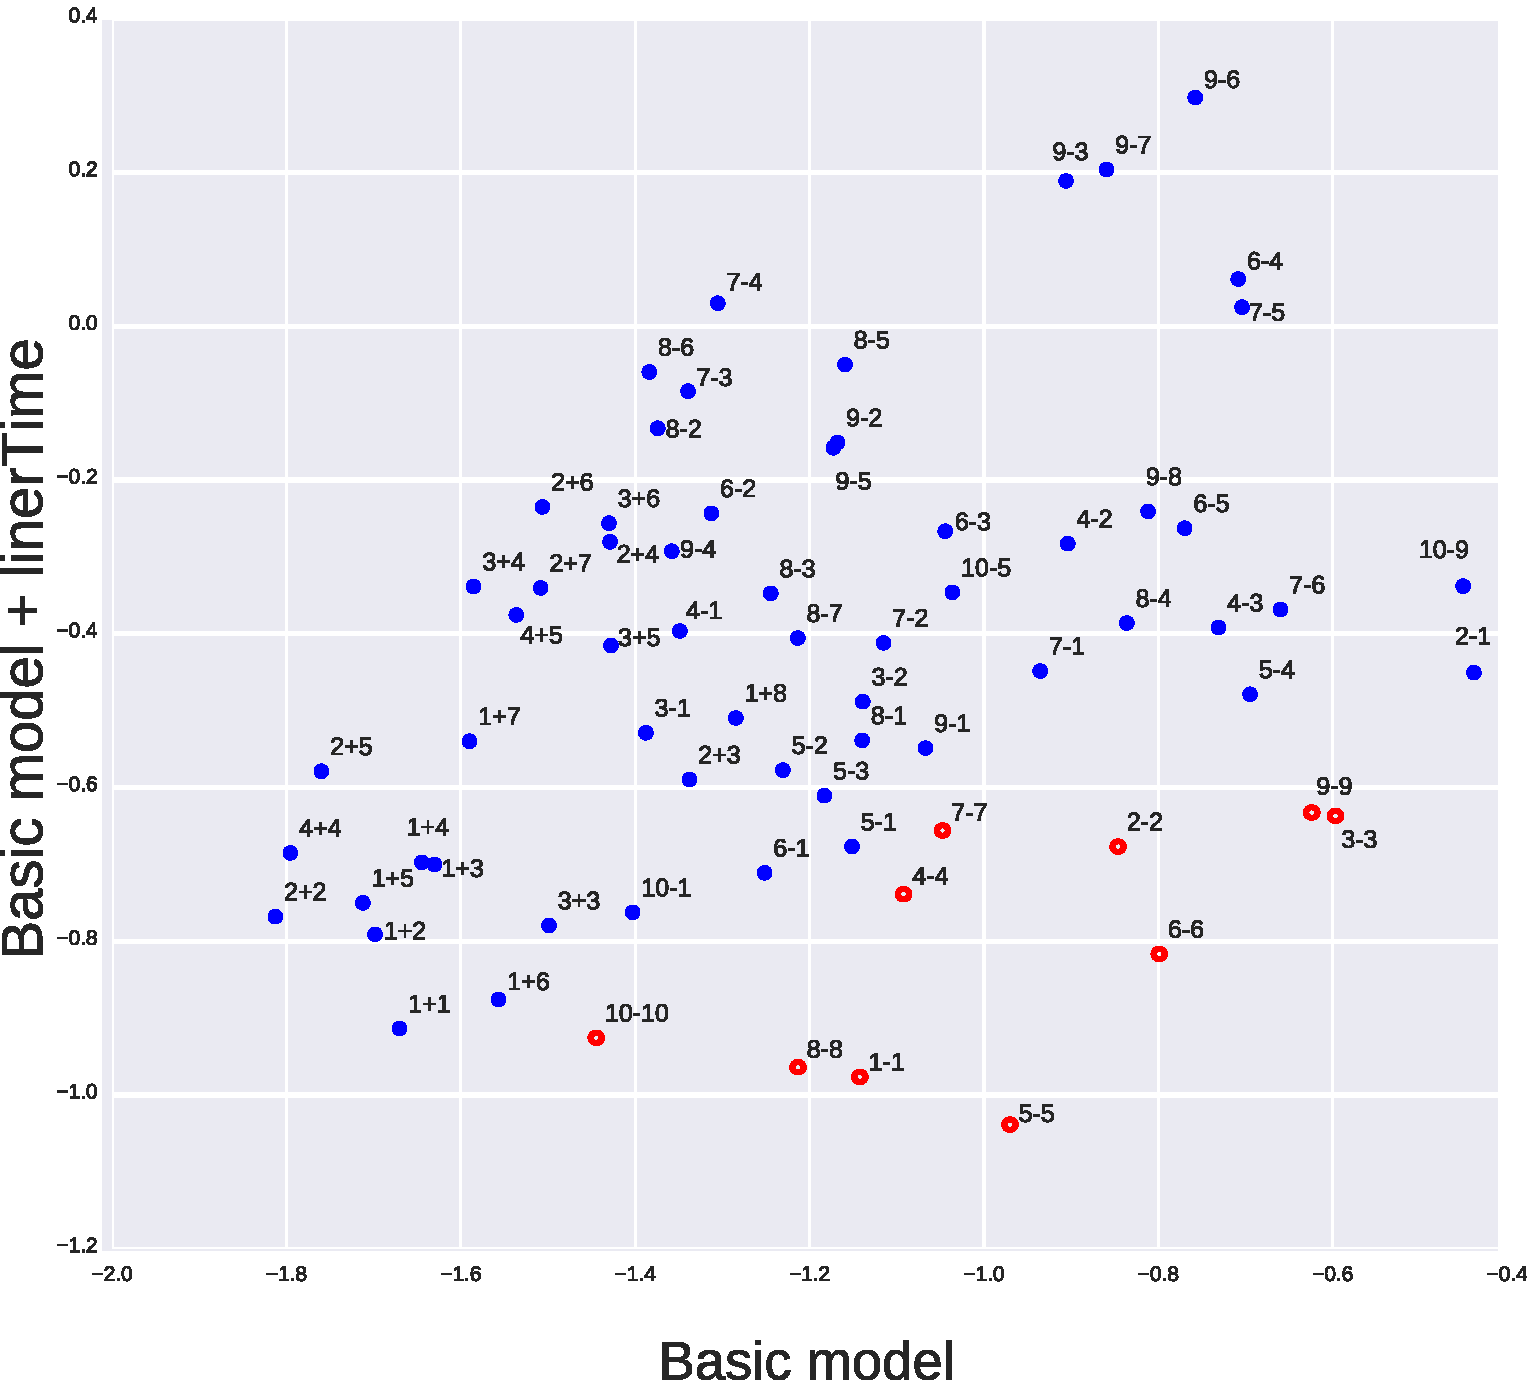
\includegraphics[width=\linewidth]{figures/difficulties}
\end{frame}
% ------------------------------------------------------------------------------
% --------------------------- SLIDE --------------------------------------------
\begin{frame}
    \frametitle{Estimated Parameters - Stability}
    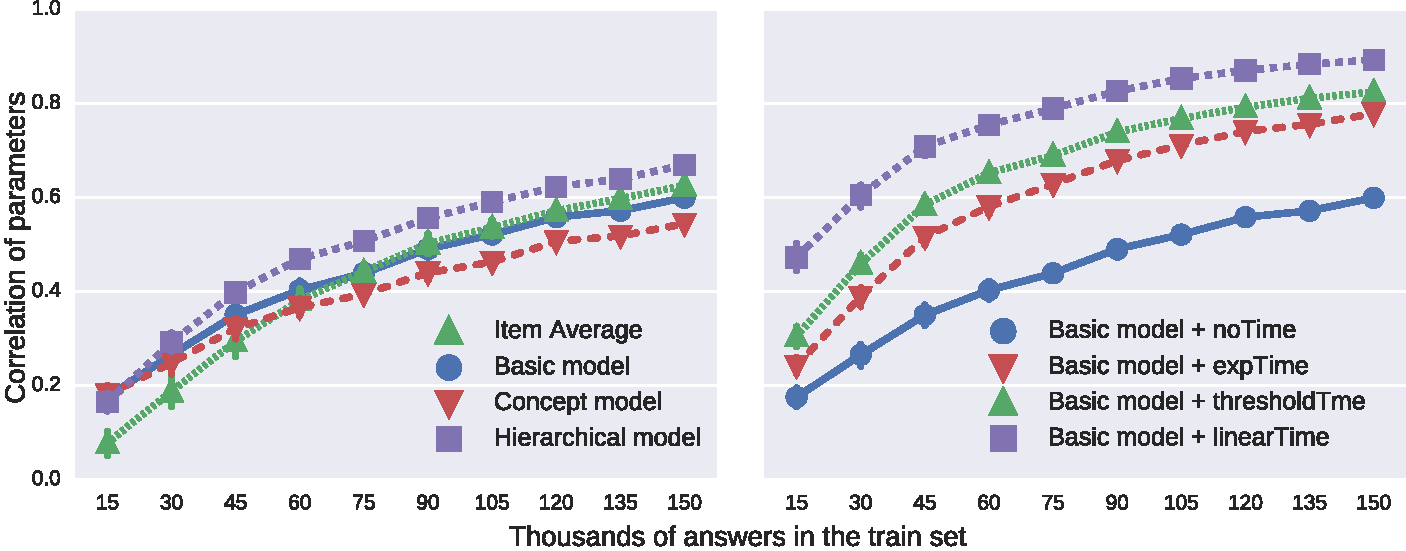
\includegraphics[width=\linewidth]{figures/stability}

    \begin{enumerate}
       \setcounter{enumi}{2}
        \item Utilization of response time have large impact on model stability.
    \end{enumerate}
\end{frame}
% ------------------------------------------------------------------------------
% --------------------------- SLIDE --------------------------------------------
\begin{frame}
    \frametitle{Conclusion}
    \begin{enumerate}
        \item Large improvement over baseline does not mean usefulness for more complex models.
        \item Response time utilization have larger impact on trained parameters that domain modeling.
        \item Utilization of response time have large impact on model stability.
    \end{enumerate}
    Incorporation of different aspects of student modeling may be more important than detailed modeling of one particular aspect.
\end{frame}
% ------------------------------------------------------------------------------


\end{document}
% ------------------------------------------------------------------------------
% ------------------------------------------------------------------------------
% ------------------------------------------------------------------------------
% --------------------------- SLIDE --------------------------------------------
\begin{frame}
    \frametitle{}
\end{frame}
% ------------------------------------------------------------------------------
\begin{itemize}
\end{itemize}